\chapter{Lab Maintenance}
\section{Rigs}
\subsection{Calibration}
Measuring equipment has to be periodically recalibrated to ensure accurate operation.  New measuring equipment must also be calibrated before use.  Calibration different types of equipment is described here.  If the equipment you are attempting to use is not described here, please check documentation that was included with the equipment and update the lab manual to reflect the new equipment.

\subsubsection{Thermocouples}\index{thermocouples!calibration}\label{sec:thermocouplecalibration}
The OPTO system is capable of reading several types of thermocouples accurately.  The lab does not have a system for cold junction compensation\index{cold junction}\index{thermocouples!cold junction}, so the zero point of the thermocouples has to be measured.  This is done by immersing each thermocouple in a container filled with ice and water.  The reading of the thermocouple on the system should now be used as the compensation value.  

In Sumulink, double click on the rig block and change the compensation value for the thermocouple in question to 0 (zero).  Check the measurement from the thermocouple and enter this value into the compensation box.  The thermocouple should now read 0\deg C.

\subsubsection{pH meters}

\subsubsection{Flow meters}

\section{Computer setup}
When a new computer is brought into the lab, there are a few things that need to be done to make it work well with the other computers.  This section covers most of the custom setup that can not be done by IT personel.  Also covered are small tasks that do not justify an IT callout.

\subsection{Jobs covered by IT}
The IT services can save a lot of time when setting up a new computer or when something has happened to a computer that is not immediately fixable by anyone in the lab.  These jobs include
\begin{itemize}
	\item Network troubleshooting
	\item Periphiral setup (new network cards)
\end{itemize}

\subsection{Registering hardware}
All valuable hardware must be registered and assigned an internal reference number `Bate nommer'.  This must be done as soon as possible to avoid misunderstandings during stocktakings.  In addition to this registration, new network cards must be assigned an IP address by IT.  To do this, obtain the MAC address of the network card by either typing \verb|ipconfig| in the windows command prompt or typing \verb|ifconfig| as root on a linux machine, then call IT and tell them that you would like to register a network device.  They will ask for the MAC address and assign an IP on the DHCP server.

\subsection{PDF printer setup}

\subsubsection{Installing the printer}
Go to the Control panel, Printers section and click on Add Printer.  Select the network printer option, entering \verb|\\groa\pdfprinter| in the printer name box.  Click next.  Windows will complain about the server not having the correct drivers and will bring up a printer driver selection box.  Select a printer with colour and PostScript capabilities (the HP Colour Laserjet XXX PS works well).

\subsubsection{Setting the properties}
Before printing, right click on the printer you have just installed and select properties.  In the dialog box that follows, click the \verb|Printing preferences| button highlighted in red in figure~\ref{fig:properties}.  
\begin{figure}
	\centering
	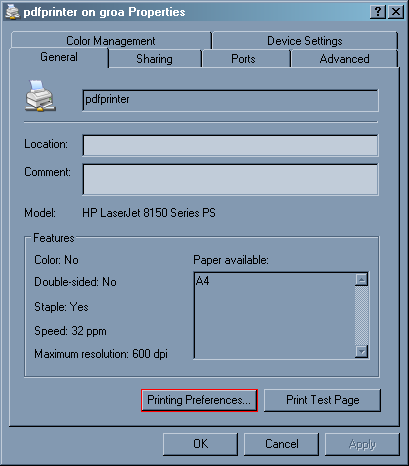
\includegraphics[scale=0.5]{properties.png}
	\caption{Printing properties dialog box}
	\label{fig:properties}
\end{figure}
Now click the \verb|Advanced| button highlighted in red in figure~\ref{fig:preferences}.  
\begin{figure}
	\centering
	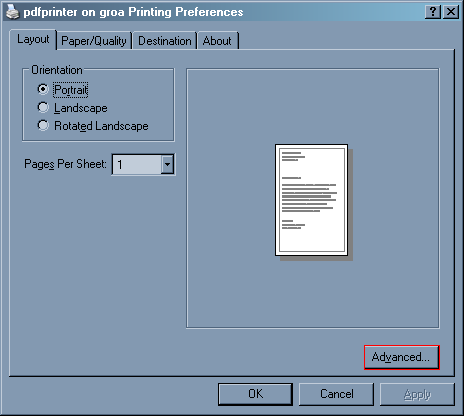
\includegraphics[scale=0.5]{preferences.png}
	\caption{Printing properties dialog box}
	\label{fig:preferences}
\end{figure}
In this advanced dialog box, make the following changes (highlighted in red on figure~\ref{fig:advanced})
\begin{figure}
	\centering
	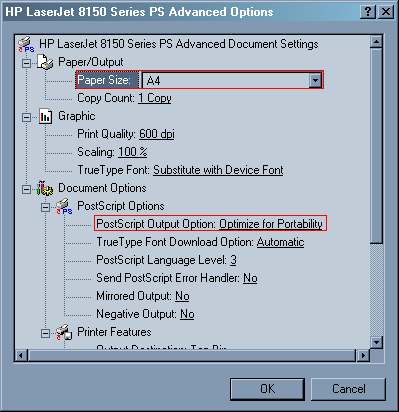
\includegraphics[scale=0.5]{advanced.png}
	\caption{Printing properties dialog box}
	\label{fig:advanced}
\end{figure}
\begin{itemize}
	\item Change the paper size to A4
	\item Click on the `Postscript Options' item in the menu to expand it and change the `Postscript output options' to `Optimize for portability'.
\end{itemize}

\subsubsection{Making a PDF}
You are now set up to make your first PDF.  Open a document in your favourite word processor and select the relevant print command\footnote{Note to Word users:  The print icon on the icon bar does not bring up a dialog box, but prints directly to the default printer -- you need to select `File/Print\dots'}.  In the dialog box that follows select the PDF printer you installed in the previous steps.  Now print normally.

\subsubsection{Getting the PDF}
The PDF will be placed in a directory shared as \verb|\\groa\PDFdrop|.  You can navigate to groa and then open this folder or you can press the windows key together with `R' and then enter the path exacly as it is typed here.  The folder will contain your PDF file with a name made up of the date and a unique job number.  Move this file to a folder on your computer and rename it to something sensible.

\section{Linux server administration}
The Linux printer server in the labs will tend to stay well-behaved most of the time.  If something does go wrong, this section will help to troubleshoot problems.  Also covered here are some basic administration commands for user maintenance